\chapter{Реализация и экспериментальная проверка}

\begin{annotation}
	В данной главе приводятся детали разработки и экспериментальной проверки
	разработанной системы. Описан выбор инструментов, используемых для реализации
	программного обеспечения. Приводится выбор инфраструктурных решений,
	с учетом поставленных ранее системных и функциональных требований.
	Описаны состав и структура реализованного программного обеспечения.
\end{annotation}


% Недостаток ~- это то, что градиент не ходит по ансамблю, а только
% внутри одной модели. Возможно, если сделать из этого одну модель
% и изучить то, как будет работать в ней обратные связи, рекурентность,
% мы можем оптимизировать вычисления и процесс обучения.


\section{Выбор инструментальных средств}
\begin{annotation}
	В данном разделе обосновывается выбор инструментальных средств с учетом выдвинутых в 3
	главе требований к системе. Рассматриваются инструменты для обработки и хранения данных,
	для разработки backend и frontend части приложения. Рассматриваются инструменты для работы
	с нейросетями и графами для реализации компонента, связанного с вычислением нейро-нечеткой системы.
\end{annotation}
% В этом разделе обосновывается выбор инструментальных средств; одним из критериев выбора могут быть какие-либо требования к разрабатываемой системе, и если этих требований много, они могут быть выделены в отдельный раздел, или же в приложение. Этот пункт не пишется, если в аналитической главе был раздел, посвященный сравнительному анализу и выбору инструментальных средств.

% В качестве системы, реализующей очереди, будет использован Python модуль aiotasks.
% Этот модуль позволяет в одном процессе запустить сразу несколько ассинхронных обработчиков задач.
% Если обработчики выполняют io-bound задачи (задачи, которые большую часть времени
% ждут операций ввода-вывода), такая архитектура может обрабатывать на порядки больше запросов,
% в сравнении с однопоточными обработчиками на io-bound классе задач.

% Для распараллеливания работы с данными и использовании аппаратных ускорений для умножений матриц
% для реализации модуля подсистемы обработки данных и подсистемы для вычисления нечеткой карты
% будет использоваться pytorch. Это фреймворк для работы с данными и созданию нейросетей.

% Кроме того, для работы с данными будет исползоваться Python-библиотека networkx. А для визуализации данных
% - matplotlib.


\section{Состав и структура реализованного программного обеспечения}
\begin{annotation}
	В данном разделе рассматривается состав и структура реализованного программного обеспечения.
	Приводятся характеристики разработанного программного продукта, возможности конфигурации отдельных
	компонент системы. Описано назначение исполняемых файлов, описаны требования к системному окружению.
\end{annotation}

Реализованное по --- это модуль на python.
Нужно прикрутить автотесты, coverage, линтеры

% Нужно охарактеризовать реализованное ПО: является ли оно настольной программной для Windows, или веб-приложением в  форме сайта/веб-сервиса, или модулем/подключаемой библиотекой, или \dots. Также нужно перечислить, из чего оно  состоит: какие исполняемые файлы и их назначение, конфигурационные файлы, файлы баз данных, требования к программному  и аппаратному окружению, и т.п.

% Если реализованное приложение достаточно обширно, этот раздел может быть
% разделен на несколько: один с общим описанием, и по одному на подсистемы самого
% верхнего уровня.


% Разработанное программное обеспечение состоит из:
% \begin{itemize}
% 	\item Подсистемы скачивания данных
% 	\item Подсистемы обработки данных
% 	\item Подсистемы для построения когнитивных картирования
% 	\item Подсистемы общения с пользователем
% \end{itemize}

% Все подсистемы работают на удаленном сервере под управлением дистрибутива ОС Linux Ubuntu.


% \section{Основные сценарии работы пользователя}

% Нужно помнить, что пользователем может быть не только <<менеджер>> или <<человек в белом халате>>, но и другой программист. Последнее относится, в первую очередь, к реализованным библиотекам. Для <<обычных>> приложений нередко бывают пользователи нескольких категорий --- например, обычный пользователь и администратор. Для каждой категории нужно описать, как выполняются основные функции, предпочтительно, с помощью серии скрин-шотов. Однако считается плохим тоном вставлять длинную вереницу из скрин-шотов: если их много, большую часть нужно выносить в приложение. Для \textit{этого} раздела нормальной является плотность скрин-шотов из расчета: 1 страница скрин-шотов на 1-2 страницы текста.

\section{Генерация тестовых данных}

Проверить качество разработанной системы можно на искусственном наборе
данных. \ref{pic:example_data_formulas}

Имеет смысл использовать искусственные данные так как мы точно знаем
зависимость между временными рядами.

\def\figurename{Формулы}
\begin{figure}[t]
	\begin{center}
	\begin{align*}
		x_1 &= sin(10t) \\
		x_2 &= 0.1 sin^2(100t) \\
		x_3 &= -0.05 cos(30t)/5 \\
		x_4 &= 0.5 t \\
		x_5 &= x_2 + x_4\\
		y   &= \frac{x_1}{5} + x_3 + x_4
	\end{align*}
	\end{center}
	\caption{Формулы, по которым генерируется искусственный набор данных}
	\label{pic:example_data_formulas}
\end{figure}
\noindent

todo мб добавить немного шума?
todo нужны числа!, а не качественный "анализ на глаз"

\section{Тестирование разработанной системы}

Для тестирования системы были построены 3 варианта карты:
\begin{itemize}
	\item Карта без связей.
	\item Полносвязная карта.
	\item Карта с осмысленными связями.
\end{itemize}

Все карты обучались 100 эпох, имели размерность скрытого состояния 100,
количество исторических данных, обрабатываемых с помощью LSTM на одной итерации -~ 100.
Так же как и количество данных на выходе, сгенерированных.

% todo таблица
% Время обучения
% Качество

Карта без связей \ref{lstmfcm_empty}, обученная на тестовых данных
показала отличный результат для $ x_1, x_2, x_3, x_4  $. Однако ошибка
для $ x_5, y $ довольно велика. Такие предсказания эквивалентны предсказаниям
отдельно взятых моделей LSTM, обученных для предсказания временного ряда
по истории только этого временного ряда.

Карта, которая представляет из себя полносвязный граф \ref{pic:lstmfcm_fc},
из-за избыточности связи получила предсказания для $ x_1, x_2, x_3 $ даже
хуже, чем карта без связей. Это можно объяснить излишней сложностью модели.
Модель слишком усложнена и не может обучиться за заданное количество эпох.

Карте с осмысленными связями \ref{lstmfcm_meaningful} удалось сохранить качество
предсказаний для $ x_1 --- x_4 $ таким же, как и у карты без связей.
А так же удалось получить улучшение предсказания для $ y $.
Неожиданный результат получили для $ x_5 $. todo как так?

Для карт, у которых были связи с $ x_5, y $ получилось лучше предсказать значения
для этих рядов. Потому что значения этих рядов зависят от $ x_1 --- x_4 $.

Кроме того, на долгосрочных предсказаниях видно, что $ x_4 $ имеет проседания.
Вероятно, это связано с ограничениями, рассмотренными во второй главе.
Так как модель обучается на одних данных, а после предсказания, модель возвращает
данные в новой области значений, будущие предсказания становятся все более нестабильными.
todo не понятно, почему их нет на предсказании LSTM

\def\figurename{Рис}
\begin{figure}
	\centering
	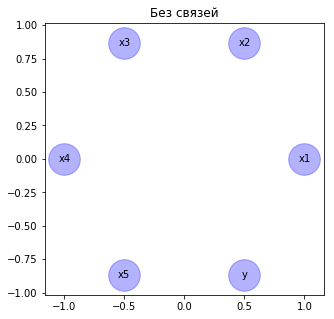
\includegraphics[width=0.7\columnwidth]{./img/lstmfcm_empty.png}
	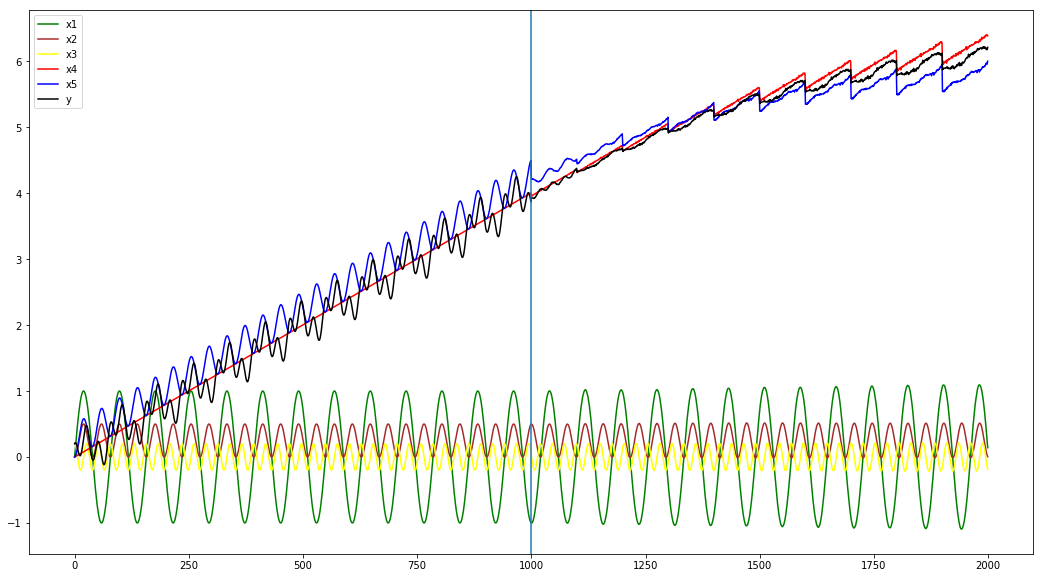
\includegraphics[width=0.9\columnwidth]{./img/lstmfcm_empty_prediction.png}
	\caption{Карта без связей концептов}
	\label{pic:lstmfcm_empty}
\end{figure}

\begin{figure}
	\centering
	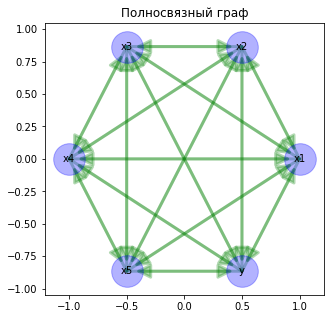
\includegraphics[width=0.7\columnwidth]{./img/lstmfcm_fc.png}
	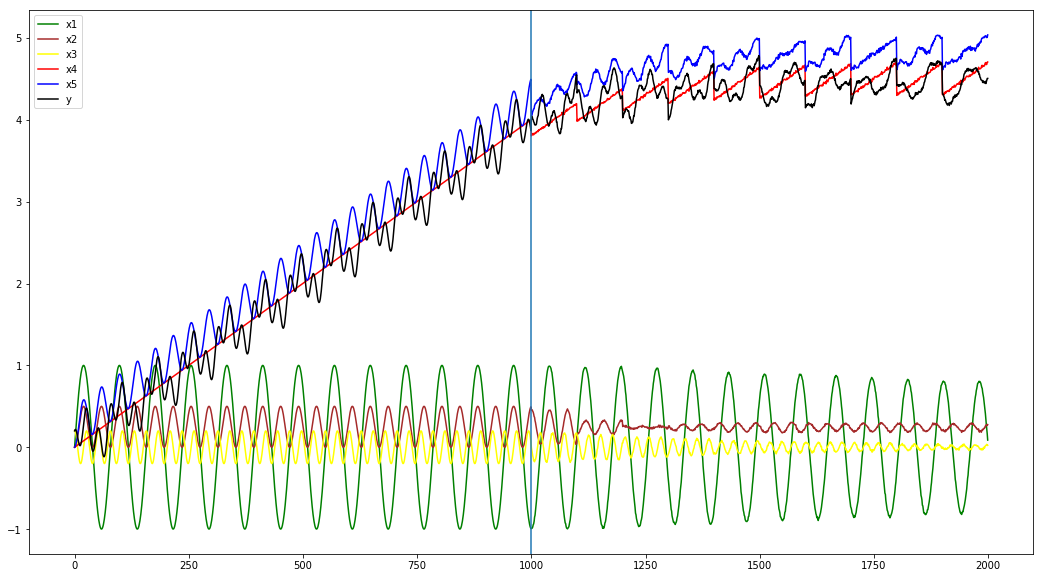
\includegraphics[width=0.9\columnwidth]{./img/lstmfcm_fc_prediction.png}
	\caption{Полносвязная карта}
	\label{pic:lstmfcm_fc}
\end{figure}

\begin{figure}
	\centering
	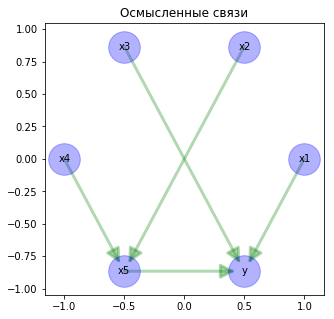
\includegraphics[width=0.7\textwidth]{./img/lstmfcm_meaningful.png}
	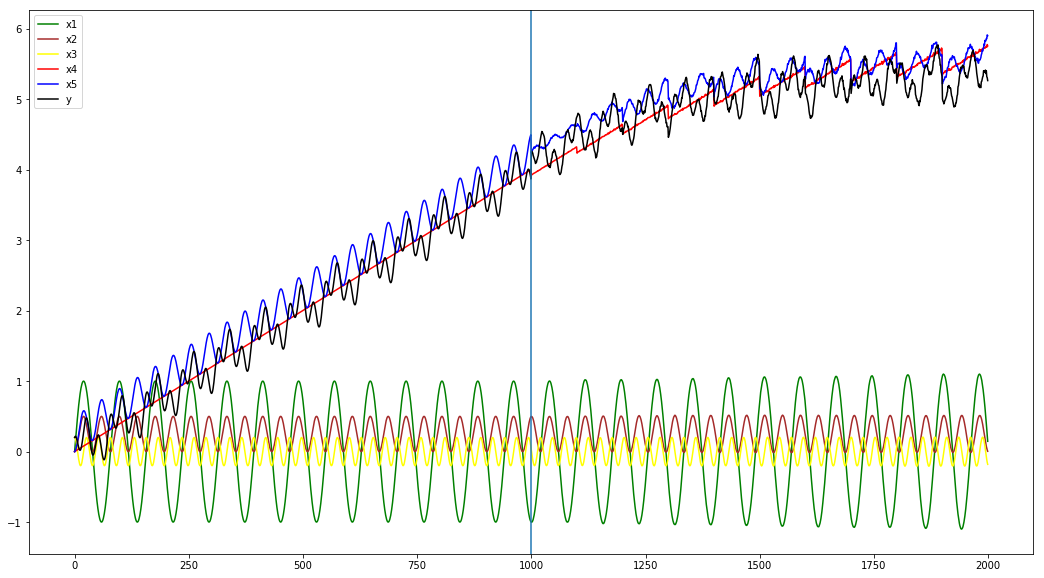
\includegraphics[width=0.9\textwidth]{./img/lstmfcm_meaningful_prediction.png}
	\caption{Карта с осмысленно расставленными связями}
	\label{pic:lstmfcm_meaningful}
\end{figure}


\section{Сравнение разработанной системы с существующими}

Была построена модель, основанная на LSTM,
которая одновременно анализирует все временные ряды тестовых данных.

Результат предсказаний такой модели представлен на рисунке \ref{lstm_only_prediction}.
Результат зашумлен по сравнению с предсказаниями карты (todo не могу объяснить).
И в отличие от карты, даже с осмысленными связями, на этом предсказании не наблюдается скачков
между итерациями предсказаний. И $ x_5 $ тоже удалось предсказать относительно успешно.

Данная модель так же, как и карта работала рекурсивно:
на каждой следующей итерации обрабатывала данные, полученые на предыдущей.
Скачок вначале предсказаний, скорее всего, связан с тем, что после обучения,
скрытое состояние сети выставляется заново, так как меняется его размерность.
Возможно, использование скрытого состояния одинаковой размерности во время
тренировки и во время тестирования, может избавить от этой проблемы. Однако
в LSTM NFCM между итерациями тоже сохраняются эти скачки, хотя между итерациями
скрытое состояние не переинициализируется.

\begin{figure}
	\centering
	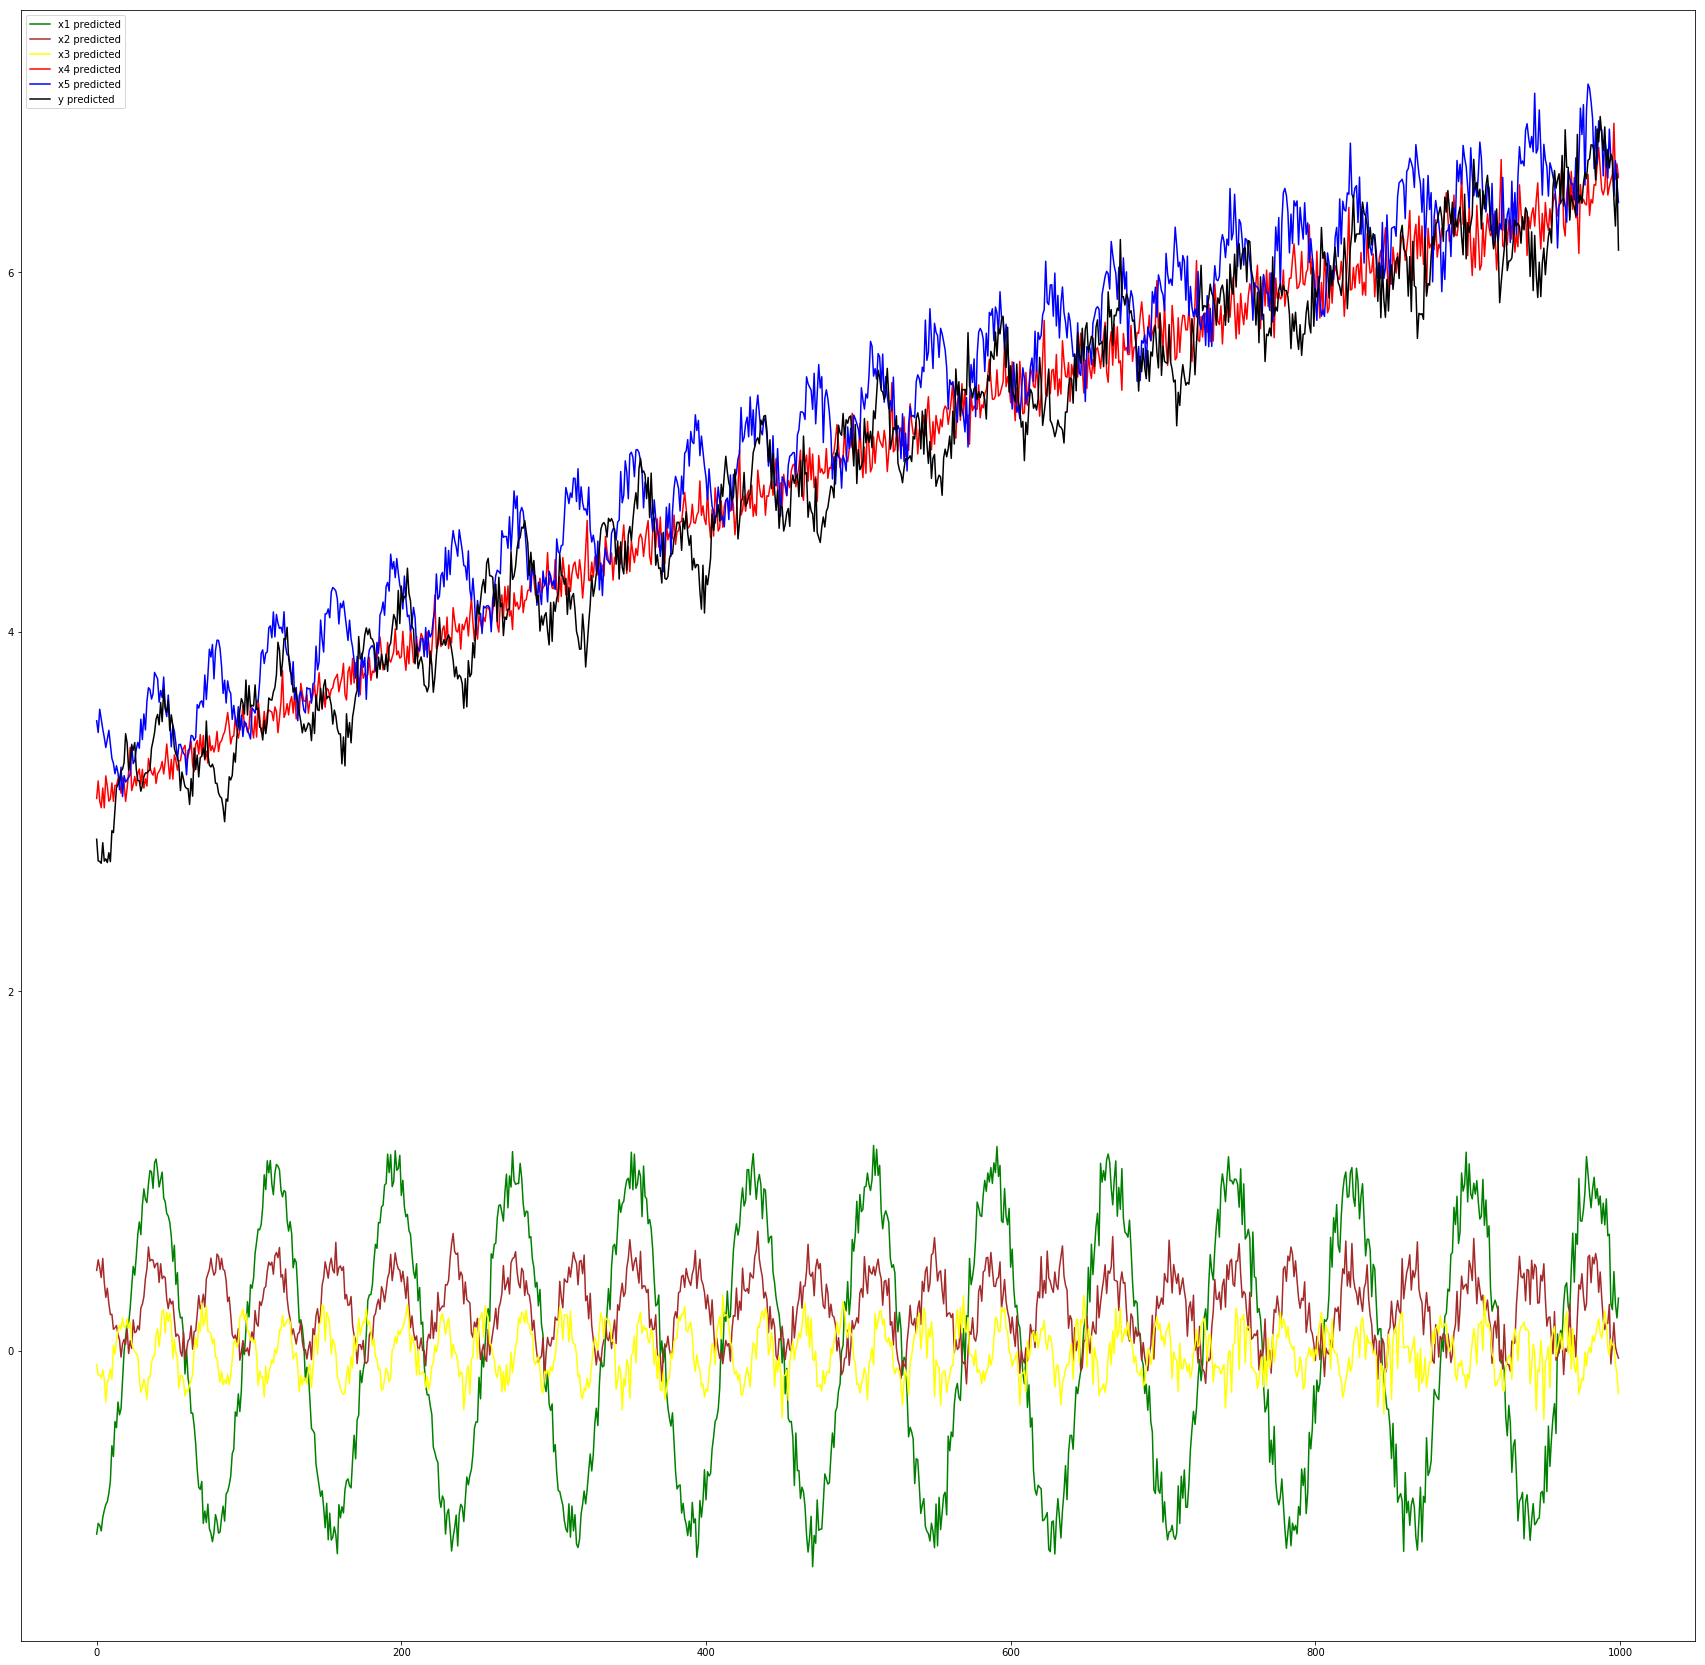
\includegraphics[width=0.9\textwidth]{./img/lstm_only_prediction.png}
	\caption{LSTM only model prediction}
	\label{pic:lstm_only_prediction}
\end{figure}


% Было реализовано несколько модификаций разрабатываемой системы, а также
% протестированы некоторые существующие системы для решения задачи прогнозирования.



\section{Влияние гиперпараметров модели на качество предсказаний}

Что, если уменьшать $ n_steps_in, n_steps_out $?
Посмотреть, как карта будет самобалансироваться, если сделать прикольную обратную связь.

При уменьшении количества эпох обучения, карта может расходиться, даже карта с осмысленными связями.

Увеличение параметра $ n_steps_in $, количество предыдущих значений временных рядов,
а так же размерность скрытого состояния увеличивают количество требуемой для обучения
памяти не более, чем линейно каждый. Конкретный показатель роста будет зависеть от
плотности связей в карте.
Уменьшение этих параметров, позволяет сэкономить память и ускорить обучение,
но страдает качество предскзаний.


\section{Моделирование с помощью разработанной системы}
\begin{annotation}
	В данном разделе описывается процесс тестирования разработанной системы.
	Описаны реализованные unit-тесты и описывается процесс функционального тестирования.
	Приводятся результаты моделирования. Проверяется то, что система соответствует выдвинутым ранее требованиям.
	Производится оценка работы системы.
\end{annotation}

\section{Выводы}

В данной главе была реализована система для автоматического когнитивного картирования с использованием
методов нейронных сетей.
Также описаны инструменты, с помощью которых была реализована система.
Описана структура программного обеспечения, проведено тестирование разработанной системы.
На основе тестирования была дана оценка реализованной системе.

% Следует перечислить, какие практические результаты были получены, а именно: какое программное или иное обеспечение было создано. В число результатов могут входить, например, методики тестирования, тестовые примеры (для проверки корректности/оценки характеристик тех или иных алгоритмов) и др. По каждому результату следует сделать вывод, насколько он отличается от известных промышленных аналогов и исследовательских прототипов.

